\section*{Overview}

Aho-Corasick is the right tool when one text must be checked against many patterns at once. It starts from a trie of
the patterns, then adds failure links so the scan through the text never needs to restart from scratch.

\section*{When to Use It}

Use Aho-Corasick when:

\begin{itemize}
  \item there are many patterns,
  \item the text is long enough that checking each pattern independently is too slow,
  \item the alphabet is manageable and pattern reuse through shared prefixes is significant.
\end{itemize}

\section*{Core Idea}

Build a trie of all patterns. Then for each node, compute a failure link to the longest proper suffix of that node's
string that is also a trie prefix. During text scanning:

\begin{itemize}
  \item follow trie edges when possible,
  \item otherwise follow failure links until a valid transition exists.
\end{itemize}

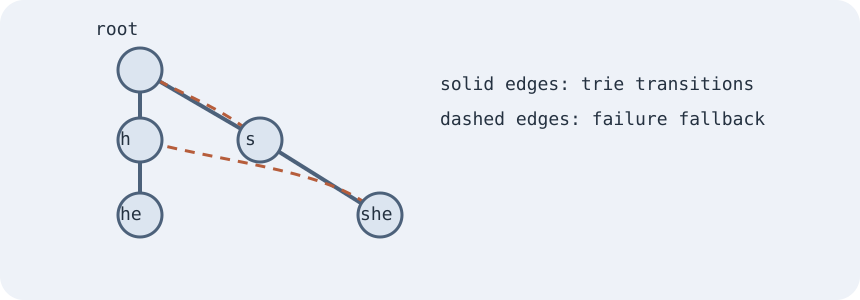
\includegraphics[width=\textwidth]{figures/failure-links.svg}

\section*{Key Insight}

The failure link is the multi-pattern analog of KMP fallback. After a mismatch, it preserves the longest suffix that is
still a valid prefix of some pattern, so already-matched text is never rescanned.

\section*{Operations / Main Technique}

\begin{itemize}
  \item insert all patterns into the trie,
  \item BFS to build failure links,
  \item scan the text once,
  \item report matches from the output list of the current state.
\end{itemize}

\paragraph{Worked example.}
If the automaton is currently at the node for \(\texttt{hers}\) and the next character breaks that path, the failure
link may jump to the node for \(\texttt{s}\), \(\texttt{rs}\), or another proper suffix prefix that still matters,
depending on the inserted patterns.

\section*{Correctness Intuition}

At every text position, the current automaton state represents the longest suffix of the processed text that is also a
trie prefix. A normal transition extends that suffix; a failure link shortens it to the next-best candidate. So every
pattern ending at the current position is eventually exposed by the output chain of the reached state.

\section*{Complexity Analysis}

If the total pattern length is \(m\) and the text length is \(n\), the construction plus scan is linear in those sizes
up to the alphabet-transition representation.

\section*{Implementation}

The code uses a lowercase alphabet trie with:

\begin{itemize}
  \item pattern insertion,
  \item failure-link construction,
  \item text scanning that counts occurrences of each pattern.
\end{itemize}

\section*{Common Pitfalls}

\begin{itemize}
  \item Forgetting to merge output information along failure links.
  \item Using the automaton when the number of patterns is tiny and simple KMP loops would be shorter.
  \item Mishandling large alphabets with a dense transition table that wastes memory.
\end{itemize}

\section*{Variants / Extensions}

\begin{itemize}
  \item Count total matches, distinct matched patterns, or first/last match positions.
  \item DP over the automaton for forbidden-substring or bounded-string construction problems.
  \item Sparse transition maps for larger alphabets.
\end{itemize}

\section*{Practice Problems}

\begin{itemize}
  \item Multi-pattern matching in one long text.
  \item Count how many times each dictionary word appears.
  \item DP on strings that must avoid a set of bad patterns.
\end{itemize}

\section*{References}

\begin{itemize}
  \item \href{https://cp-algorithms.com/string/aho_corasick.html}{cp-algorithms: Aho-Corasick}.
  \item \href{https://usaco.guide/adv/string-search}{USACO Guide: String Searching}.
  \item \href{https://codeforces.com/catalog?locale=en}{Codeforces Catalog}.
\end{itemize}
